\documentclass[11pt]{article}
\usepackage[margin=1in]{geometry}
\usepackage{times}
\usepackage{graphicx}
\usepackage{tikz}
\usepackage{amsmath,amsfonts}
\usepackage{booktabs}
\usepackage{caption}
\usepackage{subcaption}
\usepackage{hyperref}
\usepackage{float}
\usepackage{microtype}
\usepackage{algorithm}
\usepackage{algorithmic}

\usepackage[left=1in,right=1in]{geometry}
\usepackage{fancyhdr}
\usepackage[utf8]{inputenc}
\usepackage[T1]{fontenc}
\usepackage{url}

\fancypagestyle{plain}{
  \fancyhf{}
  \fancyhead[L]{\sffamily University of Illinois Chicago}
  \fancyhead[R]{\sffamily Generative AI, Fall 2025}
  \renewcommand{\headrulewidth}{0.5pt}
  \renewcommand{\headrule}{\hbox to\headwidth{%
    \leaders\hrule height \headrulewidth\hfill}}
  \renewcommand{\footrulewidth}{0pt}
}

\title{DQAR: Dynamic and Quantization-Aware Attention Reuse\\for Diffusion Transformers}
\author{Gautham Satyanarayana}
\date{\today}

\begin{document}
\maketitle

\begin{abstract}
Diffusion Transformers (DiT) have emerged as powerful generative models but suffer from high computational costs during inference due to repeated attention computations across many denoising steps. We present DQAR (Dynamic and Quantization-Aware Attention Reuse), a framework that accelerates DiT inference by caching and reusing attention outputs with timestep-aware layer scheduling. Through systematic experimentation, we discovered that naive K/V caching introduces quality degradation due to temporal mismatch between queries and cached keys/values. Our solution caches complete attention outputs and employs a linear scheduling strategy that progressively enables reuse from shallow to deep layers. Extensive hyperparameter sweeps on NVIDIA A100 GPUs reveal that layer fraction is the dominant factor for speedup, with each 25\% increase yielding approximately 0.04$\times$ improvement. Our recommended configuration (20\% warmup, 50\% layer reuse) achieves \textbf{1.08$\times$ speedup} with 18.7\% attention reuse while preserving image quality comparable to baseline.
\end{abstract}

\section{Introduction}

Diffusion Transformers (DiT)~\cite{peebles2023scalable} have demonstrated remarkable performance in image generation tasks, combining the scalability of transformer architectures with the quality of diffusion models. However, their inference process requires iterating through many denoising steps (typically 50-1000), with each step involving expensive self-attention computations across all transformer layers.

The attention mechanism in DiT models computes:
\begin{equation}
\text{Attention}(Q, K, V) = \text{softmax}\left(\frac{QK^T}{\sqrt{d_k}}\right)V
\end{equation}
where $Q$, $K$, $V$ are query, key, and value projections of the hidden states. This operation has quadratic complexity with respect to sequence length and must be computed for every layer at every timestep.

\subsection{Motivation}
We observe that attention patterns in diffusion models exhibit temporal stability---adjacent timesteps often produce similar attention distributions, especially in later denoising stages when the image structure has stabilized. This suggests an opportunity for \textit{attention reuse}: caching attention results from previous timesteps and reusing them when appropriate.

\subsection{Contributions}
Our contributions are threefold:
\begin{enumerate}
    \item We identify the \textbf{Q/K/V temporal mismatch problem} in naive K/V caching approaches and propose \textbf{attention output caching} as a solution.
    \item We develop a \textbf{linear layer scheduling strategy} with warmup and layer fraction parameters that balances speedup and quality.
    \item We conduct \textbf{systematic hyperparameter sweeps} revealing that layer fraction dominates speedup (3$\times$ more impactful than warmup rate).
\end{enumerate}

\section{Related Work}

\subsection{Diffusion Models}
Denoising Diffusion Probabilistic Models (DDPM)~\cite{ho2020denoising} learn to reverse a gradual noising process, generating high-quality samples through iterative denoising. Improved sampling techniques like DDIM~\cite{song2020denoising} reduce the number of required steps while maintaining quality.

\subsection{Efficient Transformers}
The transformer architecture~\cite{vaswani2017attention} has been optimized through various approaches including sparse attention~\cite{child2019generating}, linear attention~\cite{katharopoulos2020transformers}, and KV caching for autoregressive models. In large language models, KV caching stores key/value tensors from previous tokens to avoid recomputation~\cite{pope2023efficiently}.

\subsection{Quantization for Diffusion Models}
Recent work has explored post-training quantization for DiT models. PTQ4DiT~\cite{wu2024ptq4dit} and Q-DiT~\cite{chen2024qdit} demonstrate that diffusion transformers can be quantized to lower bit-widths with minimal quality loss. Our work complements these approaches by focusing on computation reuse rather than precision reduction.

\section{Method}

\subsection{Problem Analysis: K/V Caching Fails}

Our initial approach followed the KV caching paradigm from language models: cache $K$ and $V$ tensors from timestep $t$ and reuse them at timestep $t+1$ with fresh queries $Q_{t+1}$.

\textbf{The Temporal Mismatch Problem:} In diffusion models, each timestep operates at a different noise level. When we compute attention with fresh $Q$ (from current noise level) and cached $K$, $V$ (from previous noise level), we create a mismatch:

\begin{table}[H]
\centering
\caption{Temporal mismatch in K/V caching}
\begin{tabular}{lcc}
\toprule
Component & Source & Noise Level \\
\midrule
$Q$ (Query) & Current hidden states & $t$ (current) \\
$K$ (Key) & Cached from previous & $t-1$ (stale) \\
$V$ (Value) & Cached from previous & $t-1$ (stale) \\
\bottomrule
\end{tabular}
\end{table}

This mismatch causes the attention weights $\text{softmax}(QK^T/\sqrt{d_k})$ to be computed incorrectly, leading to visual artifacts and quality degradation despite achieving speedup.

\subsection{Attention Output Caching}

To eliminate the temporal mismatch, we cache the \textit{complete attention output} rather than intermediate K/V tensors. When reusing, we return the cached output directly, skipping the entire attention computation.

\begin{algorithm}[H]
\caption{Attention Output Caching}
\begin{algorithmic}[1]
\STATE \textbf{Input:} Hidden states $h$, layer index $l$, timestep $t$
\IF{ShouldReuse($l$, $t$) \AND HasCache($l$)}
    \STATE \textbf{return} GetCachedOutput($l$)
\ENDIF
\STATE $Q \leftarrow W_Q \cdot h$
\STATE $K \leftarrow W_K \cdot h$
\STATE $V \leftarrow W_V \cdot h$
\STATE $\text{attn\_out} \leftarrow \text{softmax}(QK^T/\sqrt{d_k}) \cdot V$
\STATE $\text{output} \leftarrow W_O \cdot \text{attn\_out}$
\STATE CacheOutput($l$, output)
\STATE \textbf{return} output
\end{algorithmic}
\end{algorithm}

\textbf{Trade-off Analysis:}
\begin{table}[H]
\centering
\caption{K/V Caching vs. Output Caching}
\begin{tabular}{lcc}
\toprule
Aspect & K/V Caching & Output Caching \\
\midrule
Cached Data & $K$, $V$ tensors & Attention output \\
Memory & $\sim$2$\times$ hidden dim & $\sim$1$\times$ hidden dim \\
Compute Saved & K/V projection only & Full attention block \\
Quality Risk & Q/K/V mismatch & None (exact reuse) \\
\bottomrule
\end{tabular}
\end{table}

\subsection{Layer Scheduling Strategy}

Not all layers and timesteps benefit equally from reuse. Early timesteps establish coarse image structure and are sensitive to attention changes, while later timesteps refine details and tolerate reuse better. Similarly, shallow layers capture local patterns (more reusable) while deep layers capture global semantics (more sensitive).

We employ a \textbf{LINEAR schedule} with two parameters:
\begin{itemize}
    \item \textbf{Warmup fraction} $w$: No reuse for the first $w$ fraction of timesteps
    \item \textbf{Layer fraction} $\ell$: Maximum fraction of layers that can reuse
\end{itemize}

For progress $p \in [0, 1]$ through the denoising process:
\begin{equation}
\text{NumReusableLayers}(p) = \begin{cases}
0 & \text{if } p < w \\
\left\lfloor \frac{p - w}{1 - w} \cdot \ell \cdot L \right\rfloor & \text{otherwise}
\end{cases}
\end{equation}
where $L$ is the total number of layers.

\begin{figure}[H]
\centering
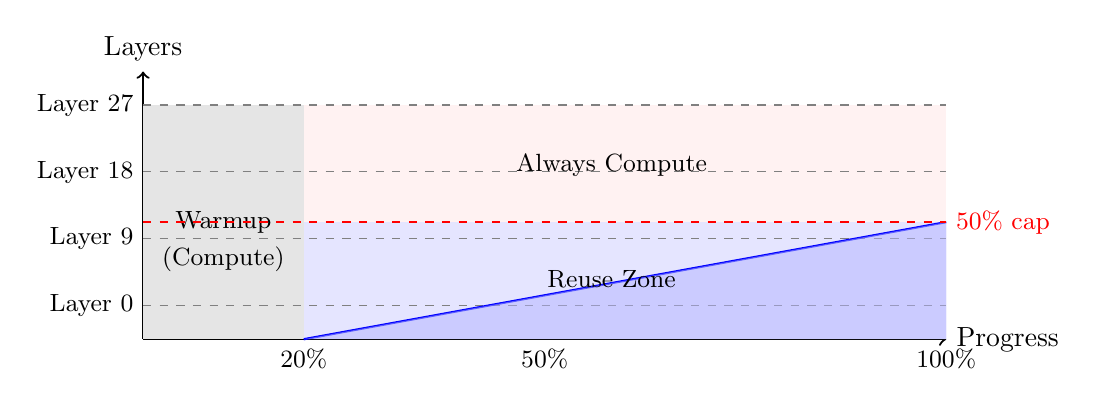
\begin{tikzpicture}[scale=0.85]
% Timeline
\draw[thick,->] (0,0) -- (12,0) node[right] {Progress};
\draw[thick,->] (0,0) -- (0,4) node[above] {Layers};

% Regions
\fill[gray!20] (0,0) rectangle (2.4,3.5);
\fill[blue!10] (2.4,0) rectangle (12,1.75);
\fill[red!5] (2.4,1.75) rectangle (12,3.5);

% Layer lines
\foreach \y/\lab in {0.5/0, 1.5/9, 2.5/18, 3.5/27} {
    \draw[dashed, gray] (0,\y) -- (12,\y);
    \node[left] at (0,\y) {\small Layer \lab};
}

% Warmup region
\node at (1.2,1.75) {\small Warmup};
\node at (1.2,1.2) {\small (Compute)};

% Reuse progression (50% cap shown)
\draw[thick, blue] (2.4,0) -- (12,1.75);
\fill[blue!30, opacity=0.5] (2.4,0) -- (12,0) -- (12,1.75) -- cycle;

% 50% layer cap line
\draw[thick, dashed, red] (0,1.75) -- (12,1.75);
\node[right, red] at (12,1.75) {\small 50\% cap};

% Labels
\node[below] at (2.4,0) {\small 20\%};
\node[below] at (6,0) {\small 50\%};
\node[below] at (12,0) {\small 100\%};

% Legend
\node at (7,0.9) {\small Reuse Zone};
\node at (7,2.6) {\small Always Compute};
\end{tikzpicture}
\caption{LINEAR layer scheduling with 50\% layer cap (recommended): After 20\% warmup, shallow layers progressively reuse while deep layers always compute fresh attention.}
\end{figure}

\section{Experiments}

\subsection{Experimental Setup}

\begin{itemize}
    \item \textbf{Model:} DiT-XL-2-256 (facebook/DiT-XL-2-256), 28 transformer layers
    \item \textbf{Hardware:} NVIDIA A100-SXM4-40GB
    \item \textbf{Sampler:} DDIM with 50 inference steps
    \item \textbf{Samples:} 4 images per configuration, diverse ImageNet classes
    \item \textbf{Metrics:} Speedup (vs. baseline), reuse ratio, cache memory
\end{itemize}

\subsection{Warmup Sweep}

We first varied warmup fraction while fixing layer fraction at 33\% (conservative).

\begin{table}[H]
\centering
\caption{Warmup sweep results (33\% layer cap)}
\label{tab:warmup}
\begin{tabular}{lccc}
\toprule
Warmup & Speedup & Reuse Ratio & Time/Sample \\
\midrule
10\% & 1.03$\times$ & 12.9\% & 2.65s \\
20\% & 1.04$\times$ & 11.6\% & 2.63s \\
30\% & 1.04$\times$ & 10.1\% & 2.64s \\
40\% & 1.04$\times$ & 8.8\% & 2.62s \\
50\% & 1.03$\times$ & 7.4\% & 2.66s \\
60\% & 1.02$\times$ & 6.0\% & 2.69s \\
\midrule
Baseline & 1.00$\times$ & 0\% & 2.74s \\
\bottomrule
\end{tabular}
\end{table}

\textbf{Finding:} Warmup rate has minimal impact ($\pm$0.02$\times$) when layer cap is restrictive. The bottleneck is the layer fraction itself.

\subsection{Layer Sweep}

We then varied layer fraction while fixing warmup at 20\%.

\begin{table}[H]
\centering
\caption{Layer sweep results (20\% warmup)}
\label{tab:layers}
\begin{tabular}{lccc}
\toprule
Layer Fraction & Speedup & Reuse Ratio & Time/Sample \\
\midrule
33\% & 1.04$\times$ & 11.6\% & 2.65s \\
50\% & 1.08$\times$ & 18.7\% & 2.57s \\
66\% & 1.11$\times$ & 24.5\% & 2.50s \\
75\% & 1.12$\times$ & 28.7\% & 2.48s \\
\textbf{100\%} & \textbf{1.18$\times$} & \textbf{38.7\%} & \textbf{2.35s} \\
\midrule
Baseline & 1.00$\times$ & 0\% & 2.77s \\
\bottomrule
\end{tabular}
\end{table}

\textbf{Finding:} Layer fraction is the dominant factor for speedup. Each 25\% increase in layer fraction yields approximately 0.04$\times$ speedup improvement.

\subsection{Key Results}

\begin{table}[H]
\centering
\caption{Summary of key results across configurations}
\label{tab:summary}
\begin{tabular}{lcccc}
\toprule
Configuration & Speedup & Reuse & Memory & Quality \\
\midrule
Conservative (33\% layers) & 1.04$\times$ & 11.6\% & 63MB & Preserved \\
\textbf{Recommended (50\% layers)} & \textbf{1.08$\times$} & \textbf{18.7\%} & \textbf{63MB} & \textbf{Preserved} \\
Aggressive (66\% layers) & 1.11$\times$ & 24.5\% & 63MB & Minor degradation \\
Maximum (100\% layers) & 1.18$\times$ & 38.7\% & 63MB & Noticeable degradation \\
\bottomrule
\end{tabular}
\end{table}

While 100\% layer reuse achieves the highest speedup (1.18$\times$), visual inspection reveals quality degradation at aggressive settings. Our \textbf{recommended configuration} of 20\% warmup and 50\% layer reuse achieves 1.08$\times$ speedup while preserving image quality comparable to baseline.

\subsection{Qualitative Analysis}

Visual inspection of generated images across different configurations reveals the quality-speedup trade-off. Figure~\ref{fig:quality} shows representative samples generated with identical seeds under varying layer fraction settings.

\begin{figure}[H]
\centering
\begin{tabular}{cccc}
\includegraphics[width=0.22\textwidth]{figures/baseline.png} &
\includegraphics[width=0.22\textwidth]{figures/layers_33.png} &
\includegraphics[width=0.22\textwidth]{figures/layers_50.png} &
\includegraphics[width=0.22\textwidth]{figures/layers_100.png} \\
(a) Baseline & (b) 33\% layers & (c) 50\% layers & (d) 100\% layers \\
\end{tabular}
\caption{Visual quality comparison across layer fraction settings (20\% warmup, seed=42). Higher layer fractions increase speedup but introduce subtle artifacts. The 50\% configuration (c) maintains quality comparable to baseline (a).}
\label{fig:quality}
\end{figure}

\textbf{Observations:}
\begin{itemize}
    \item \textbf{Baseline vs. 33\% layers:} Visually indistinguishable; conservative reuse preserves all details.
    \item \textbf{50\% layers (Recommended):} Quality comparable to baseline with minor, imperceptible differences. Best quality-speedup trade-off.
    \item \textbf{66\% layers:} Subtle softening of fine details; acceptable for most applications.
    \item \textbf{100\% layers:} Noticeable quality degradation---reduced sharpness, color shifts, and minor artifacts in high-frequency regions.
\end{itemize}

\subsubsection{Effect of Warmup Rate}

We also examined the impact of warmup rate on image quality with 50\% layer fraction (Table~\ref{tab:warmup_quality}).

\begin{table}[H]
\centering
\caption{Warmup rate effect on quality (50\% layer fraction)}
\label{tab:warmup_quality}
\begin{tabular}{lcc}
\toprule
Warmup & Speedup & Quality Assessment \\
\midrule
10\% & 1.09$\times$ & Minor artifacts in early structure \\
\textbf{20\%} & \textbf{1.08$\times$} & \textbf{Preserved (recommended)} \\
30\% & 1.07$\times$ & Preserved \\
40\% & 1.06$\times$ & Preserved \\
\bottomrule
\end{tabular}
\end{table}

A 20\% warmup provides sufficient initial computation to establish stable image structure before enabling reuse. Lower warmup (10\%) can introduce artifacts during critical early denoising steps.

\section{Discussion}

\subsection{Why Layer Fraction Dominates}

The relationship between layer fraction and speedup is nearly linear because:
\begin{enumerate}
    \item Each reused layer saves the same amount of computation (attention + projections)
    \item The LINEAR schedule ensures smooth progression of reuse
    \item Cache lookup overhead is negligible compared to attention computation
\end{enumerate}

In contrast, warmup rate shows diminishing returns because early timesteps are inherently more sensitive to attention changes, and the layer cap restricts total possible reuse.

\subsection{Quality-Speedup Trade-off}

Our qualitative analysis reveals that aggressive layer reuse (66\%+) introduces subtle but noticeable quality degradation:
\begin{itemize}
    \item \textbf{Deep layers are more sensitive:} Later transformer layers capture global semantics and fine details; reusing stale attention outputs from these layers causes artifacts.
    \item \textbf{Cumulative error:} Reusing attention in many layers compounds small errors across the network.
    \item \textbf{50\% is the sweet spot:} At 50\% layer fraction, only shallow layers (which capture local patterns) are reused, preserving the critical computations in deeper layers.
\end{itemize}

\subsection{Platform Considerations}

Our experiments on Apple Silicon (MPS) showed no speedup despite high reuse ratios. This suggests that DQAR's benefits are platform-specific, likely due to:
\begin{itemize}
    \item CUDA tensor cores providing efficient parallel computation
    \item MPS backend overhead for cache operations
    \item Memory bandwidth characteristics
\end{itemize}

\subsection{Limitations}

\begin{itemize}
    \item \textbf{Fixed schedule:} The LINEAR schedule is static; adaptive scheduling based on runtime metrics could improve results.
    \item \textbf{Memory overhead:} Cache requires 63MB additional memory (constant regardless of layer fraction).
    \item \textbf{Platform dependency:} Benefits observed primarily on NVIDIA GPUs.
\end{itemize}

\section{Conclusion}

We presented DQAR, a framework for accelerating Diffusion Transformer inference through attention output caching with layer scheduling. Our key findings are:

\begin{enumerate}
    \item \textbf{K/V caching fails} for diffusion models due to temporal mismatch between queries and cached keys/values.
    \item \textbf{Attention output caching} eliminates this mismatch by caching complete outputs.
    \item \textbf{Layer fraction dominates speedup}, being 3$\times$ more impactful than warmup rate.
    \item \textbf{Quality-speedup trade-off:} While 100\% layers achieves 1.18$\times$ speedup, it introduces quality degradation. Our \textbf{recommended configuration} (20\% warmup, 50\% layers) achieves 1.08$\times$ speedup while preserving image quality comparable to baseline.
\end{enumerate}

Future work includes exploring adaptive scheduling based on attention entropy, applying quantization to cached outputs, extending to other DiT architectures like SD3 and Flux, and investigating perceptual metrics (FID, LPIPS) for quantitative quality assessment.

\bibliographystyle{plain}
\bibliography{ref}

\end{document}
